
\documentclass[10pt,a4paper]{article}

%%%%%%%%%%%%%%%%%%%%%%%%%%%%%%%%%%%%%%%%%%%%%%%%%%%%%%%%
%
% Packages and Theorem Environments

\usepackage{graphicx}
\usepackage{psfrag}
\usepackage{epsf}
\usepackage{amsmath,amsfonts,amssymb,latexsym}
\usepackage{enumitem}
\usepackage{algorithmic}
\usepackage{algorithm}
\usepackage[width=160mm,height=240mm,left=35mm,foot=10mm]{geometry}
\usepackage{xcolor}
\usepackage{url}
\usepackage{hyperref}
\usepackage{tikz}



\renewcommand{\theequation}{\thesection.\arabic{equation}}
\newcommand{\makeTiny}[1]{{\tiny #1}}
\newcommand{\work}{\tiny}
\newcommand{\ignore}[1]{}
\newcommand{\startClaims}{\setcounter{claim}{0}}
\newtheorem{theorem}{Theorem}[section]
\newtheorem{corollary}[theorem]{Corollary}
\newtheorem{lemma}[theorem]{Lemma}
\newtheorem{proposition}[theorem]{Proposition}
\newtheorem{conjecture}[theorem]{Conjecture}
\newtheorem{problem}[theorem]{Problem}
\newtheorem{question}[theorem]{Question}
\newtheorem{definition}[theorem]{Definition}
\newtheorem{task}[theorem]{Task}
\newtheorem{claim}{Claim}
\newtheorem{remark}[theorem]{Remark}
\newtheorem{observation}[theorem]{Observation}

\graphicspath{hw2}



\title{MATH 351--004 -- Assignment \#$2$\\
}

\author{Alex Iacob\\
ai9388}

\date{September 9, 2021}


%%%%%%%%%%%%%%%%%%%%%%%%%%%%%%%%%%%%%%%%%%%%%%%%%%%%%%%%
%
% Author's definitions


\newcommand{\NN}{\mathbb N}
\newcommand{\ZZ}{\mathbb Z}
\newcommand{\QQ}{\mathbb Q}
\newcommand{\RR}{\mathbb R}

\newcommand{\BB}{\mathcal B}
\newcommand{\ZT}{\mathcal Z}

\newcommand{\Cl}{\operatorname{Cl}}
\newcommand{\Bd}{\operatorname{Bd}}
\newcommand{\row}{\operatorname{row}}
\newcommand{\col}{\operatorname{col}}
\newcommand{\Span}{\operatorname{span}}
\newcommand{\convhull}{\operatorname{conv.hull}}
\newcommand{\tr}{\operatorname{tr}}

\newcommand{\diam}{\operatorname{diam}}

\begin{document}

\maketitle

\begin{center}
{\bf \large Part 2}
\end{center}

\subsection*{Problem 1.22 - Let $G$ be a disconnected graph. By Theorem 1.11, $\bar{G}$ is connected. Prove that $u$ and $v$ are any two vertices of $\overline{G}$, then $d_{\overline{G}} (u, v) = 1$ or  $d_{\overline{G}} (u, v) = 2$. Therefore, if $G$ is a disconnected graph, then $diam(\overline{G}) \leq\ 2$.
}

Case 1: $u$ and $v$ are not adjacent in Graph $G$: \\
	$u$ and $u$ will be adjacent in comp of G with a length of 1 ($d_{\overline{G}} (u, v) = 1$). \\	
Case 2: $u$ and $v$ are adjacent in Graph $G$: \\
	$u$ and $v$ are now not adjacent, but there is a path of length 2 $d_{\overline{G}} (u, v) = 2$. \\
	
Using both of these cases would lead to the diameter either being 1 or 2 for $\overline{G}$.
\subsection*{Problem 1.24 - Determine whether the graphs $G_{1}$ and $G_{2}$ of Figure 1.34 are bipartite. If a graph is bipartite, then redraw it indicating the partite sets; if not, then give an explanation as to why the graph is not bipartite.
}
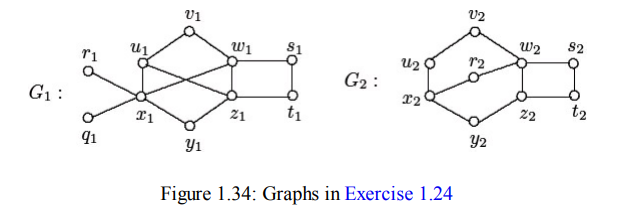
\includegraphics[width=10cm]{fig134}\\

$G_{1}: Set A is shown with circled vertices\\ 
A = \{r_{1}, q_{1}, r_{1}, y_{1}, w_{1}, t_{1}\} \\ 
B = \{x_{1}, v_{1}, z_{1}, s_{1}\}$\\
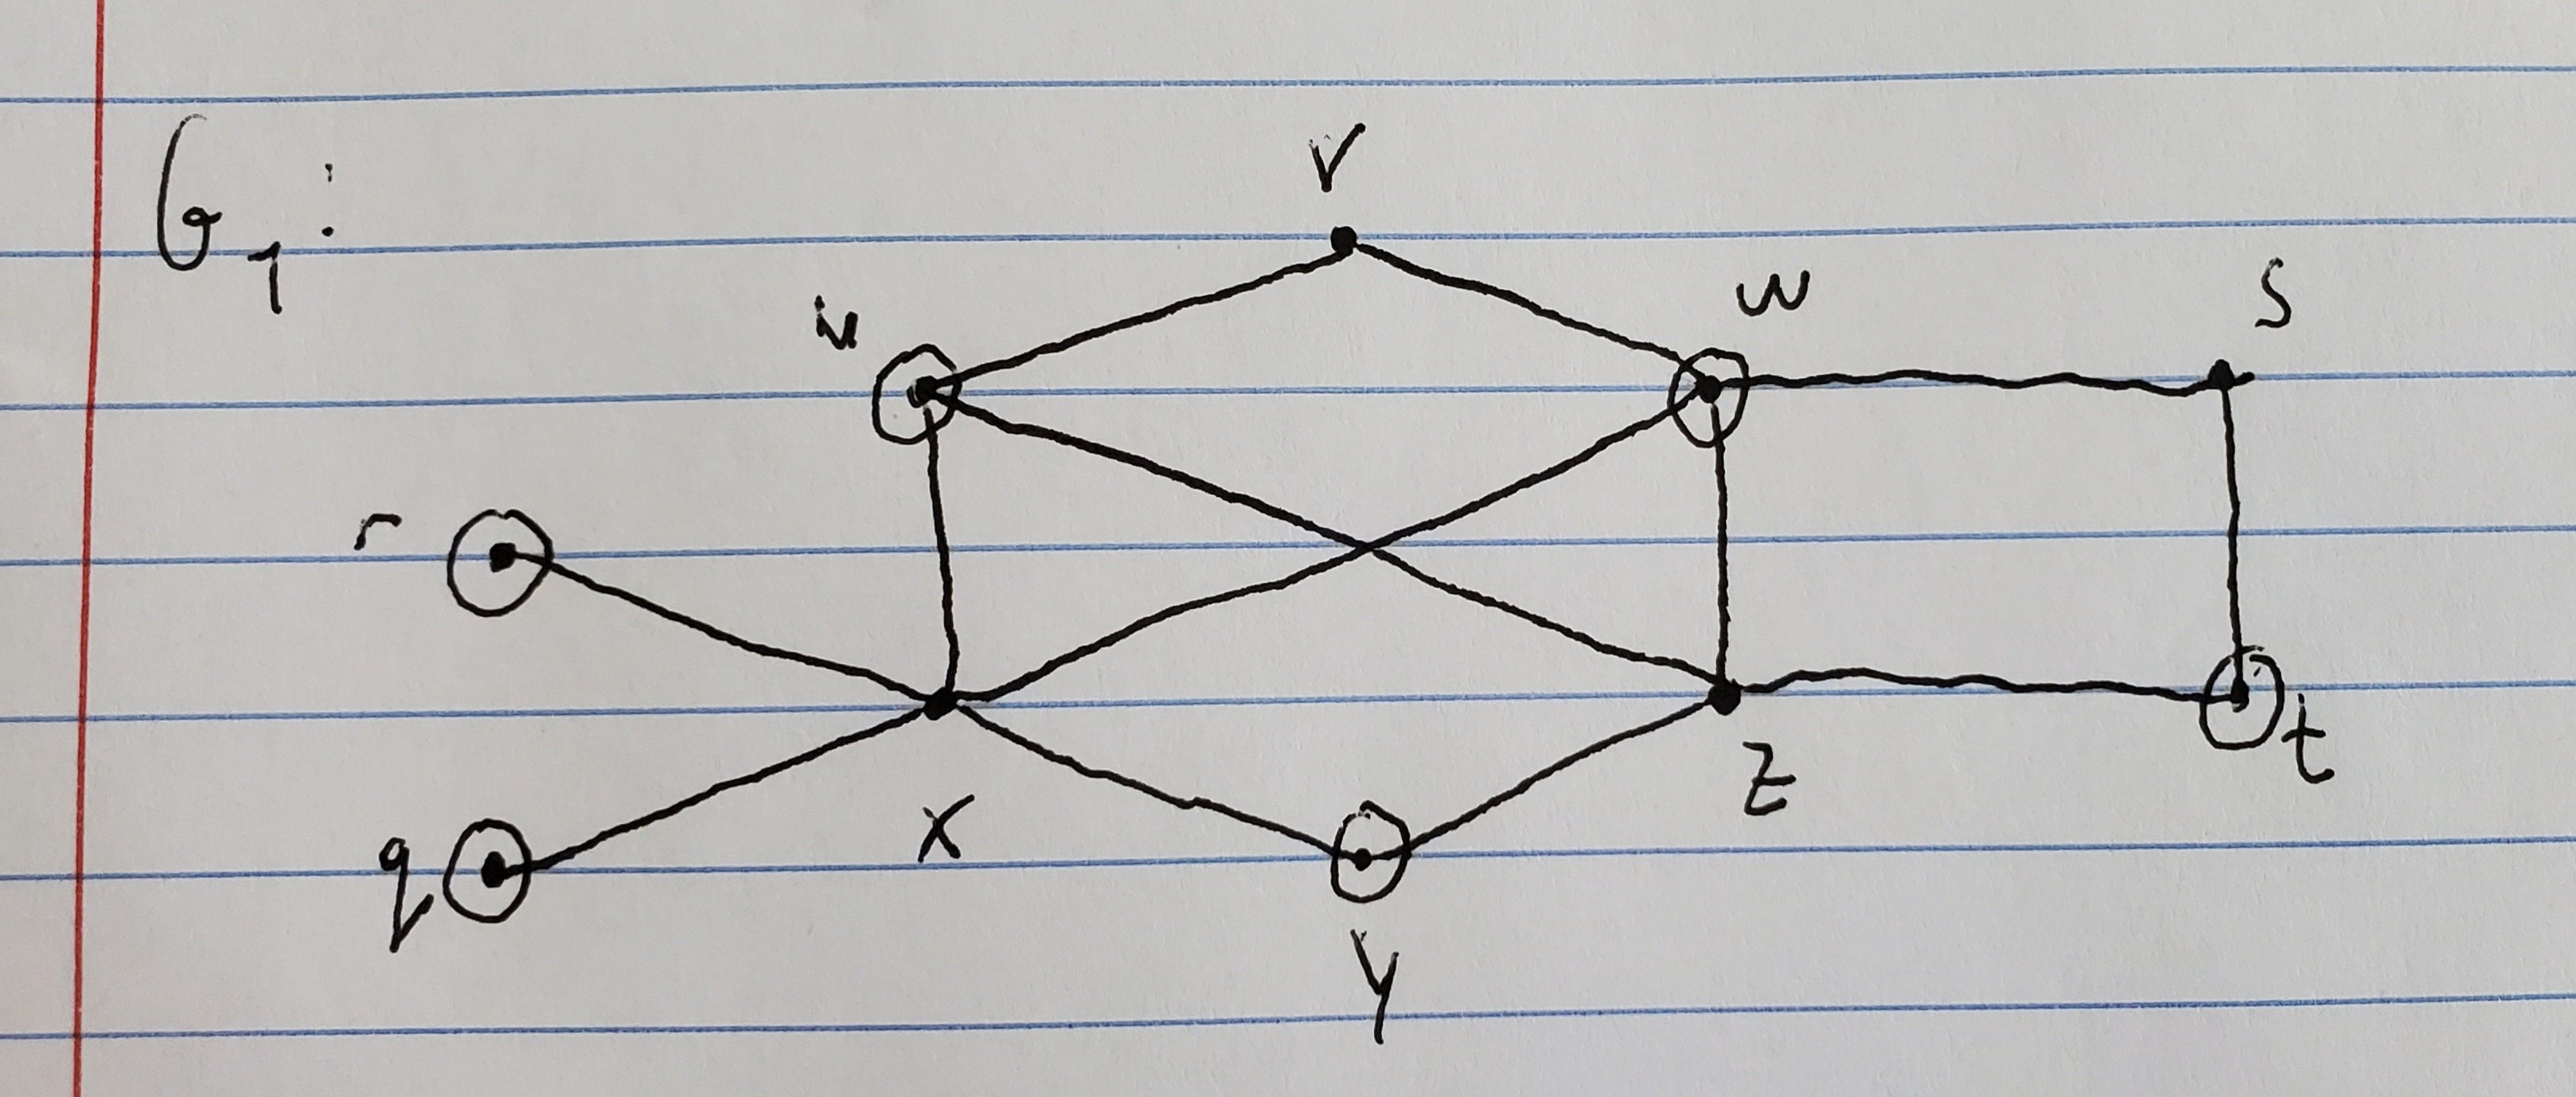
\includegraphics[width=10cm]{answerg1}

$G_{2}$ is not bipartite. It is not bipartite because it cannot be separated into bi-partitions. Using separate patterns to demonstrate.\\
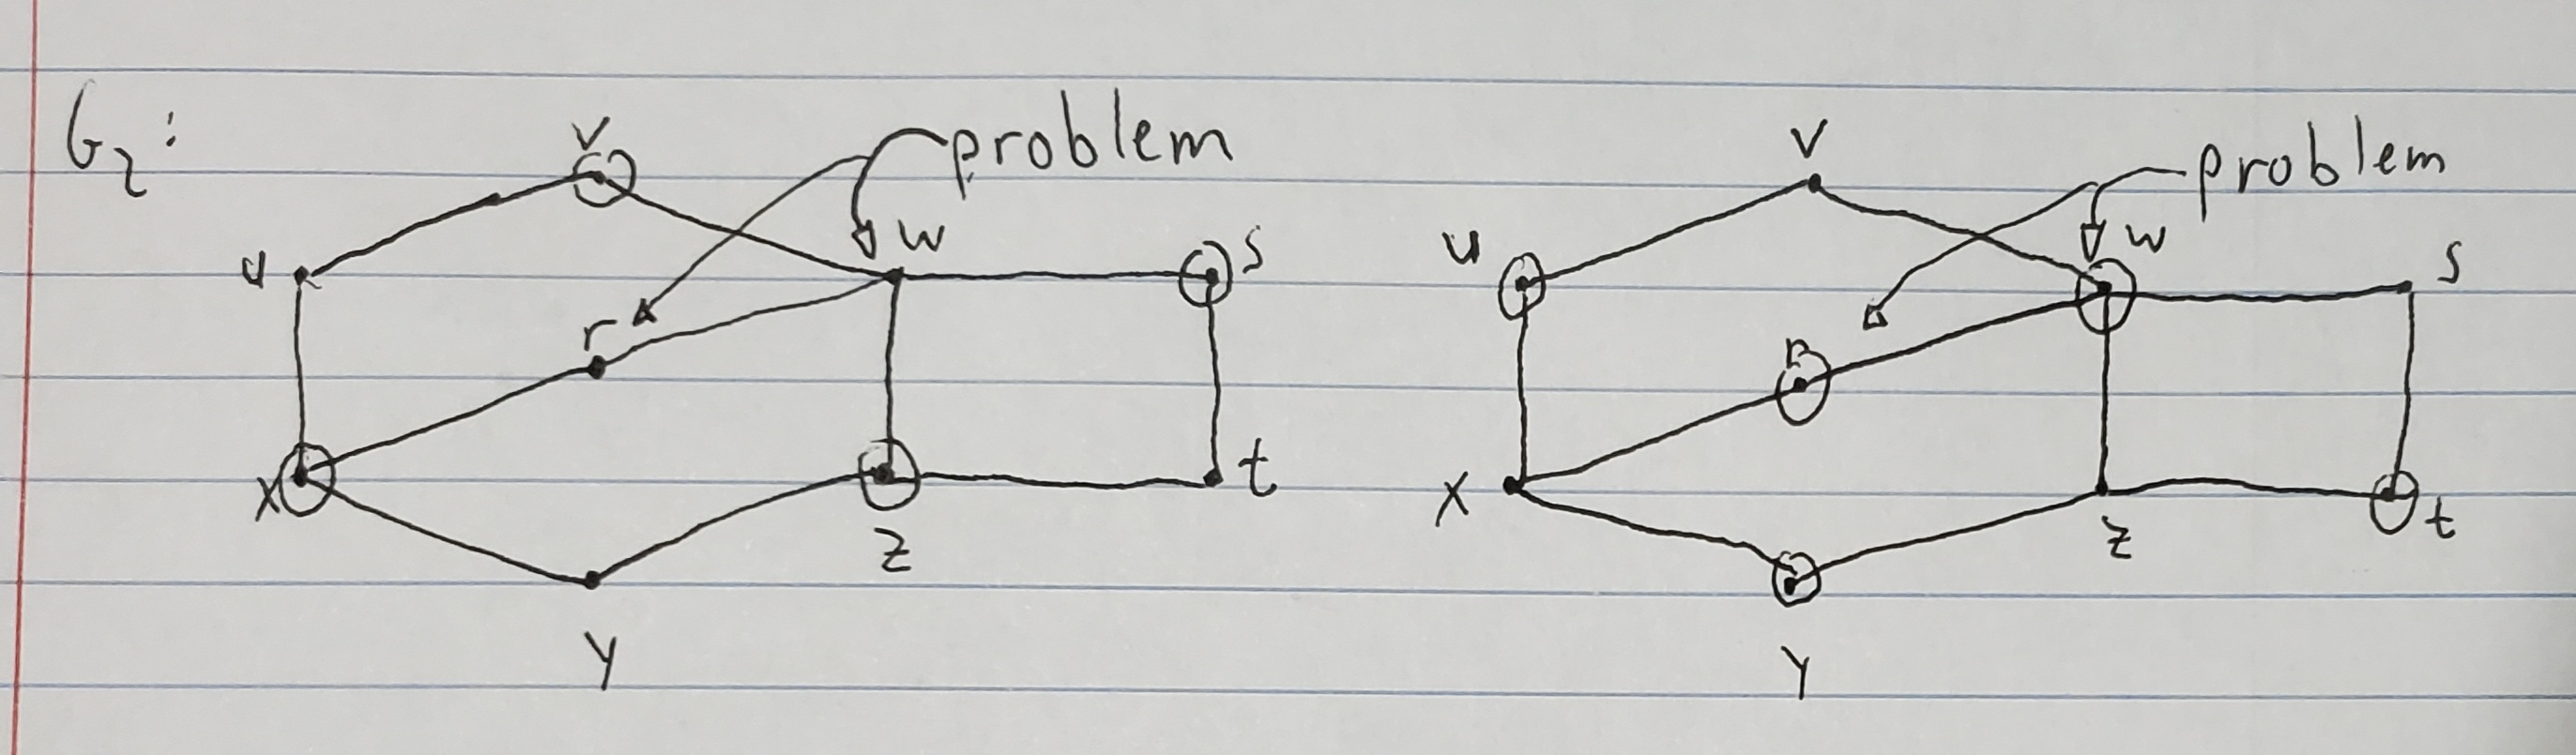
\includegraphics[width=15cm]{answerg2}

\subsection*{Problem 2.12 - Prove that if $G$ is a graph of order $n$ such that \\$\Delta (G) + \delta (G) \geq\ n - 1$, then $G$ is connected and $diam(G) \leq\ 4$. Show that the bound $n - 1$ is sharp.
}

For all $deg(u) = \Delta(G)$ and $deg(v) = \delta(G)$. Using an argument from Theorem 2.4, $deg(u) + deg(v) \leq n - 1$.
Suppose $u$ has the greatest degree in Graph $G$, $deg(u) = \Delta(G)$ and $v$ is a vertex that is not u,$v \epsilon V(G) / \{u\}$. Since we know that $deg(u) = \Delta(G)$ and $deg(v) = \delta(G)$, we can say $deg(u) + deg(v) = \Delta(G) + \delta(G)$. Thus, $d(u, v) \leq 2$.\\
The distance between any vertices (x and y for the sake of demonstration) is at most distance 2 from vertex $u$, 
$d(x, u) \leq 2$ and $d(u, y) \leq 2$. This creates two paths, one from $x$ to $u$ and another from $u$ to $y$. Now using Theorem 1.6, there is a walk from $x$ to $y$ with a distance of at most 4. 

It is shown that $n-1$ is sharp because anything less than that would leave Graph $G$ disconnected. For example, if we were to consider having $n-2$ nodes, the graph would be disconnected. 

\subsection*{Problem 2.20 Show that if G is a connected graph that is not regular, then G contains adjacent vertices $u$ and $v$ such that $deg(u) \ne deg(v)$.
}

If Graph $G$ is not regular, then that means that all the graph's vertices do not have the same degree. If we create a path between two vertices of different degrees, then somewhere along that path, there will be two adjacent vertices which satisfy $deg(u) \ne deg(v)$.

\end{document} 




















